\documentclass[12pt, a4paper]{article}

%% Text related
\usepackage[utf8]{inputenc}
\usepackage{indentfirst}
\usepackage[bottom]{footmisc}
\usepackage{verbatim} %Adds comment blocks & code copy-paste
\usepackage[ngerman, num]{isodate} %Proper date format ffs...
    \monthyearsepgerman{}{}
    \daymonthsepgerman{}{}
\usepackage{enumitem}
\usepackage{lipsum} %Because why not?
\usepackage{lscape}

\usepackage[paper=A4,pagesize]{typearea}
\usepackage{afterpage}

%% Figure related
\usepackage{graphicx}
\usepackage{float} 
\usepackage{subfig}
\usepackage[justification=centering]{caption} %Centers multiline captions

%% Drawing stuff
\usepackage{pgfplots}
\usepackage[american]{circuitikz}

%% Math & Scientific notations
\usepackage{amsmath}
\usepackage{amssymb} %amsmath doesn't have quite common math symbols for some reason
\usepackage[per-mode=repeated-symbol, tight-spacing=true]{siunitx}

%% Table related
\usepackage{multirow}
\usepackage{tabularx}
\usepackage[thinlines]{easytable} %convenient
\usepackage{booktabs} %for different horizontal lines
\usepackage{array} %for table corners not meeting up - doesn't appear to work though

%%
\usepackage{subfiles}

% pgfplots configurations
\graphicspath{ {../img/} }
\pgfplotsset{
    compat=newest,
    standard/.style={
    axis x line=middle,
    axis y line=middle,
    every axis x label/.style={at={(current axis.right of origin)},anchor=west},
    every axis y label/.style={at={(current axis.above origin)},anchor=south}
    }
}

% To place e.g. [ V ] so I don't bother typing it
\newcommand{\unitV}{{\;[\,\SI{}{\volt}\,]}}
\newcommand{\unitmA}{{\;[\,\SI{}{\milli\ampere}\,]}}
\newcommand{\unitA}{{\;[\,\SI{}{\ampere}\,]}}
\newcommand{\unitohm}{{\;[\,\SI{}{\ohm}\,]}}
\newcommand{\unitkohm}{{\;[\,\SI{}{\kilo\ohm}\,]}}

% \title{EED 3009 ENGINEERING DESIGN - II\\FEASIBILITY REPORT}
% \author{Abdurrahman ÜZÜM}
% \date{\today}




\begin{document}

    \begin{titlepage}
        \begin{center}

            \begin{figure}

                \subfloat
                {%
                    
\includegraphics[width=0.3\textwidth]{deulogo.png}
                }
                %
                \hfill
                %
                \subfloat
                {%
                    
\includegraphics[width=0.3\textwidth]{facultylogo.png}
                }

            \end{figure}

            \textbf{T.C.\\}
            \textbf{DOKUZ EYLUL UNIVERSITY\\}
            \textbf{ENGINEERING FACULTY\\}

            \vspace*{1 cm}
            \textbf{ELECTRICAL \& ELECTRONICS ENGINEERING\\}
            \textbf{DEPARTMENT\\}

            \vspace*{1 cm}
            \textbf{EED3009 ENGINEERING DESIGN - II\\}
            \textbf{THEORETICAL DESIGN REPORT\\}

            \textbf{RANGE FINDER}

            \vspace*{1 cm}

        
            \begin{table}[H]\centering
                \begin{tabular}{cc}
                    Elif Sezin ÖZYİĞİT \hspace{1cm}  & \hspace{1cm} Abdurrahman ÜZÜM \\
                    2019502098         \hspace{1cm}  & \hspace{1cm} 2019502099       \\             
                \end{tabular}
            \end{table}

            Instructor:\\ Dr.Ogr.Uy.Neslihan AVCU\\

            \vspace*{1 cm}
            December, 2022


        \end{center}

    \end{titlepage}

    \pagebreak
    
    \tableofcontents

    \pagebreak

    \begin{abstract}
        Early societies measured distance with a variety of primitive tools, from basic paces to measuring rods and marked ropes.\cite{abstract} Luckily, we’ve come a long way from the days of using belts, thumbs and cubits for measurement. Various methods have been developed over the years in order to increase the measurement accuracy and to be able to measure in various conditions. These devices, which have been developed by human beings step by step over the years and evolved with new technologies, have reached the level where they can measure without the need for physical contact or even light.
    \end{abstract}

    \section{Introduction}

        This project focuses on measuring distances with no contact up to a meter. To realise this project a battery powered, handheld device will be designed. The device will utilise an ultrasonic speaker and microphone. It will send regular periodic ultrasonic bursts from the speaker and listen for the echoes. The necessary circuitry will measure the time between sent ultrasonic bursts and their respective echoes, following the time of flight (ToF) principle. This data will then be processed using necessary information such as the speed of sound on air, as a result of which, the distance data will be obtained. Finally, this distance value will be printed on a two digit display. The device will also employ a laser guide to assist proper alignment of the sensors, and also to provide a feedback to the user. 


    \section{Objectives of the Project}

        \noindent The designed device must follow the above guidelines and accomplish these aims. 
        \begin{itemize}
            \item Measure distances in the range of 0-99\SI{}{\centi\metre}
            \item Indicate if the distance is over the range.
            \item Have an accuracy of \SI{1}{\centi\metre}
            \item Be battery powered and handheld
            \item Display the measured distance in real time on a two digit display.
            \item Not empoly an MCU or ASIC designed for this particular purpuse.
        \end{itemize}

        \noindent In terms of measurement accuracy and range, the given properties can evolve as the experiments and tests continue, and therefore are subject to change. 

        
    \pagebreak
    \section{Overview of the Project}

        \begin{figure}[H]\centering
            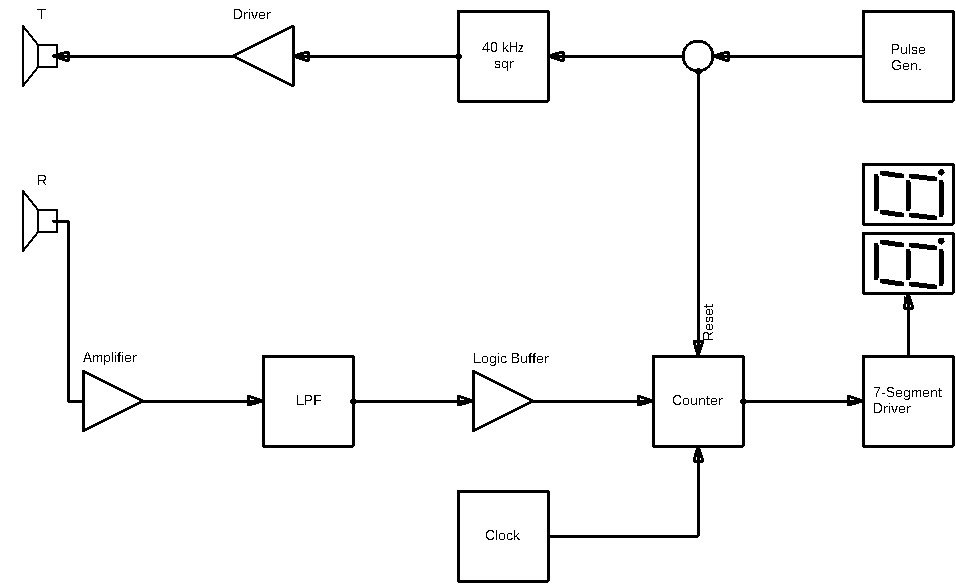
\includegraphics[width = \textwidth]{schematics/blockdiagram_v3.png}
            \caption[]{Revised Block Diagram}
        \end{figure}

        \bigskip
        Guidelines of distance measurement using ultrasonic sensors is relatively straight forward. All the device should do is to send sound signals, wait for the echoes arrive and measure the time between. Since transmitting a continuous signal would produce a continuous echo, it is not possible to keep track of the time. Therefore the transmitter should emit bursts of sound waves, and the receiver should keep track of the time between.

        \bigskip 
        Two ultrasonic transducers are needed, one for the transmitter and one for the receiver. The transmitter should be driven periodically with short pulses. The timing between these pulses is critical, such that the following pulse should not be transmitted before the echo of the previous pulse has arrived. This calculation should be made in consideration of the longest distance to be measured. Width of these pulses is also critical, as it should be short enough to ensure that the echo doesn't arrive before the pulse ends. This calculation should be made in considetation of the shortest distance of interest. 
    

    \pagebreak    
    \section{Design and Methodology}
        
        This section contains schematics of the blocks in the block diagram. Given below is the entire schematic of the system. The design is confirmed with simulations which will be discussed later on the Results section. Design is almost finalized and most likely will not see any significant changes. Minor changes are still possible, see discussion secsion for a summary of the encountered problems. Note that due to the image dimention problems, 7-segment display and overrange indication LED are not shown in this schematic. 

        \noindent Each block of the schematic will be explained below in detail.

        \bigskip\bigskip

        \begin{figure}[H]\centering
            \makebox[\linewidth]
                {
                    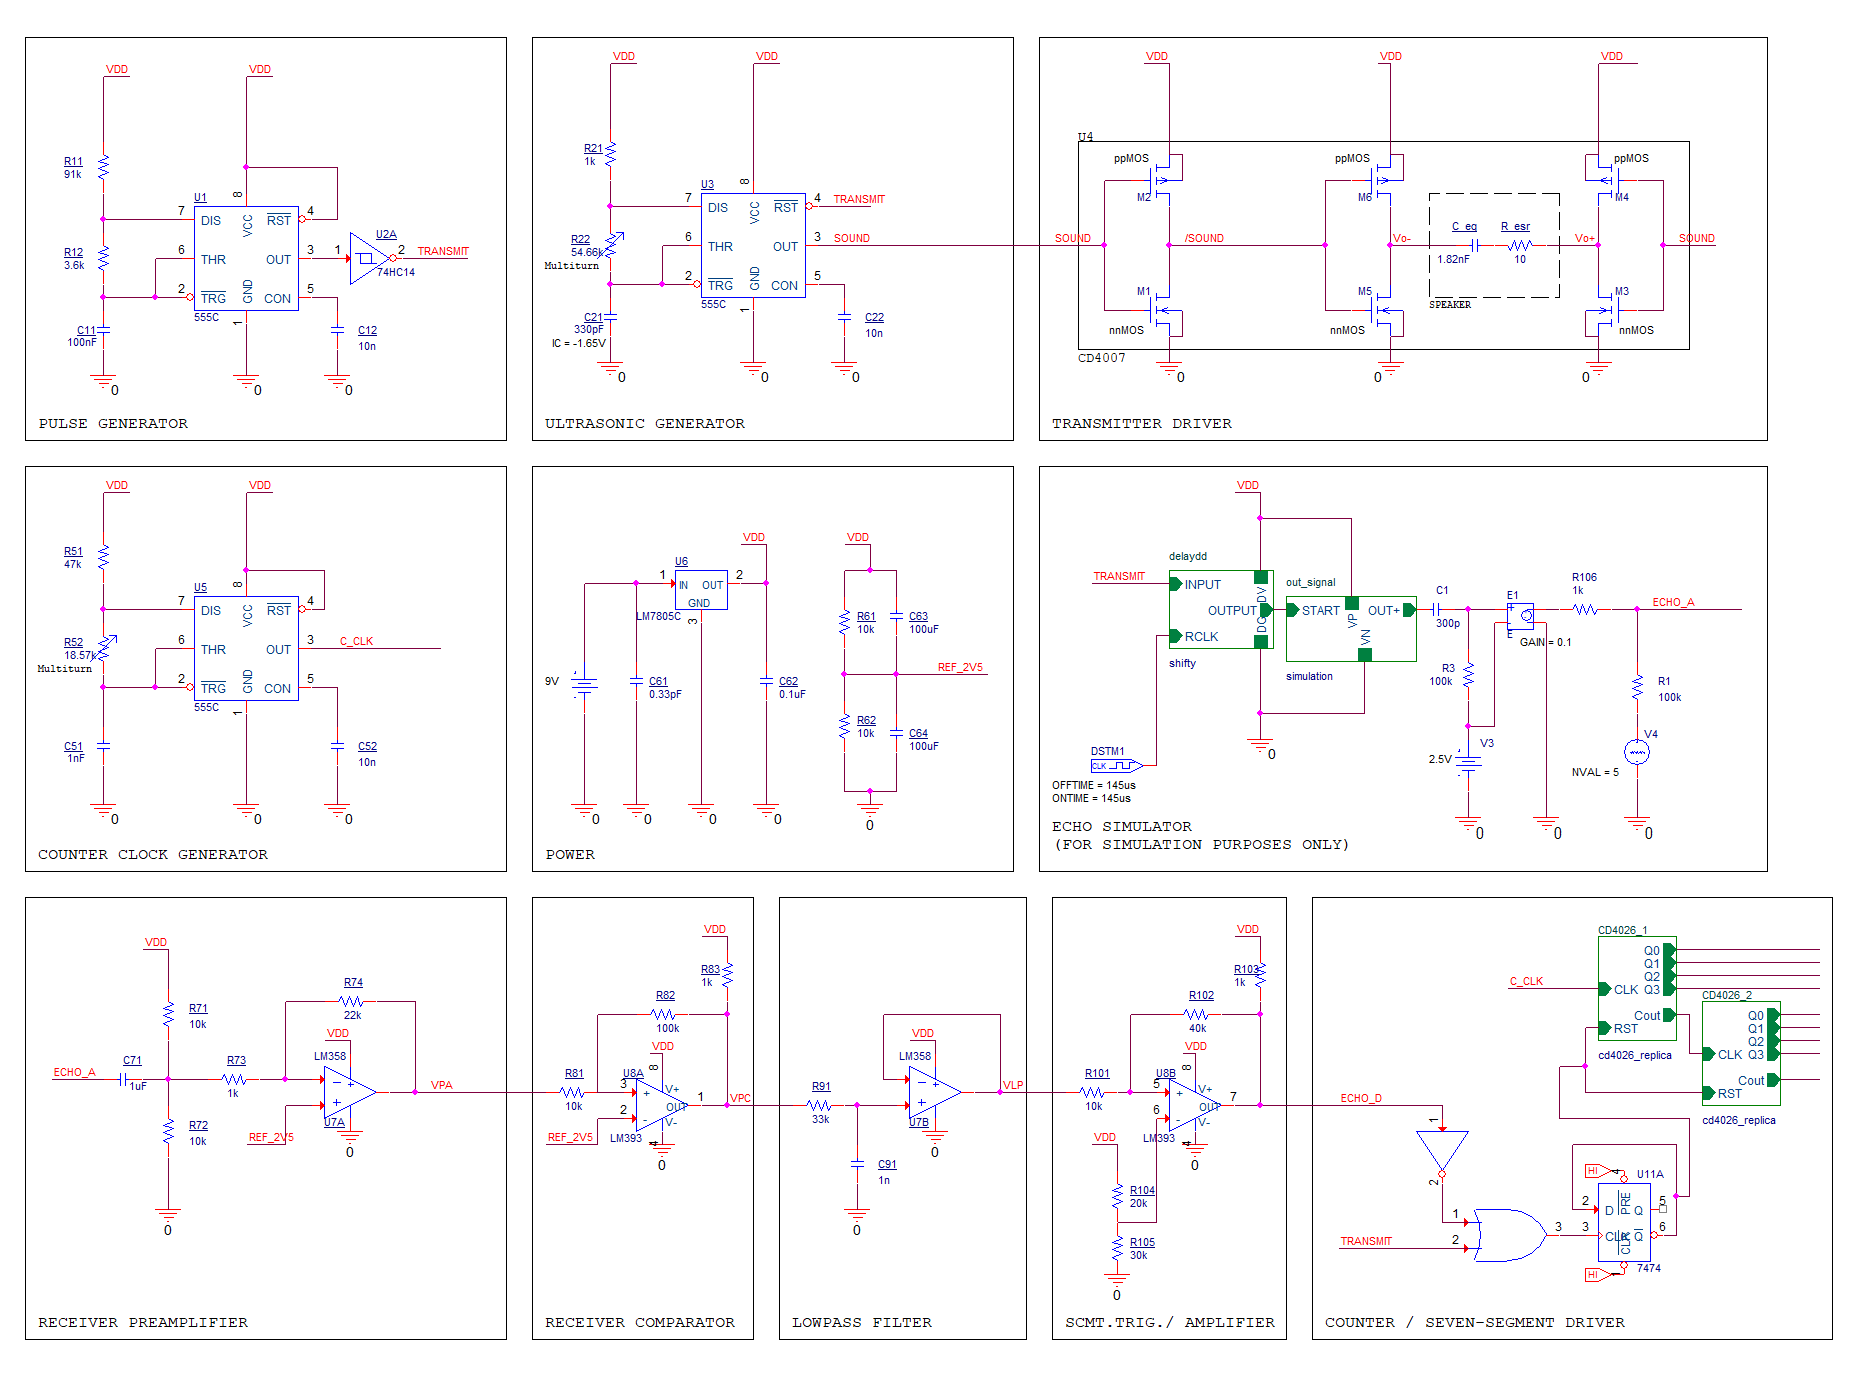
\includegraphics[width=1.3\linewidth]{schematics/complete.png}
                }
                \caption[]{}
        \end{figure}

    
    	\subsection{Ultrasonic Frequency Synthesis}

            \begin{figure}[H]\centering
                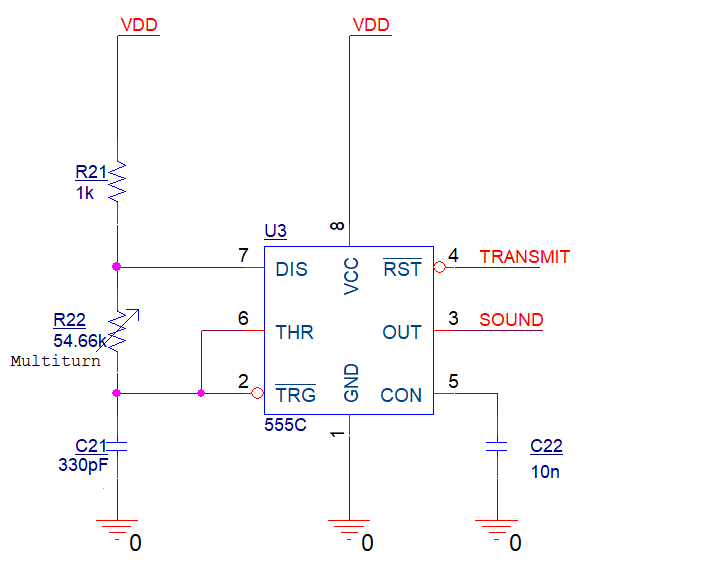
\includegraphics[width=0.75\textwidth]{schematics/ultra_gen.png}
                \caption[]{}
            \end{figure}
	
	        Commonly available ultrasonic transducers work at frequencies near \SI{40}{\kilo\hertz} as tested and confirmed by the experiment in the feasibility report. Therefore the transmitter should send bursts of \SI{40}{\kilo\hertz} sound waves that fill the pulses. In order to provide a signal with these properties, two generators are needed. One to generate the \SI{40}{\kilo\hertz} signal, and another to generate the pulses.
            
            \bigskip 
            Synthesizing sinusoidal waves is rather involved and hard. This is usually done digitally by the help of microcontrollers. Since this project does not allow the use of microcontrollers, and there are no readily available sinusoidal signal generator IC’s, it has been decided that driving the transmitter with square waves will suffice. This is also how the HCSR04 module was operating. Refer to the feasibility report Section 4 Figure 5.

            This ultrasonic signal will be generated using a 555 timer in astable mode. Using the equations provided on datasheet
            
            \begin{equation}\begin{aligned}
                T = 0.693(R_A + 2R_B)C &= \num{25e-6} \\
                         (R_A + 2R_B)C &= \num{36.1e-6} \\
                          R_A + 2R_B   &= \num{109e3}
            \end{aligned}\end{equation}

            \noindent Let $C$ = \SI{330}{\pico\farad} and $R_A$ = \SI{1}{\kilo\ohm}

            \begin{equation}
                \implies R_B = \SI{54.16}{\kilo\ohm} 
            \end{equation}

            \noindent Since the transducers are most likely to operate in a relatively narrow range of frequencies, for optimal performance, the signal should be kept close to \SI{40}{\kilo\hertz}, therefore to accurately set timing, a \SI{5}{\kilo\ohm} trimpot can be added in series with \SI{51}{\kilo\ohm} resistor in place of $R_B$.

            As can be seen from the scheamtic, RESET input of the 555 timer is connected to a net called ``TRANSMIT''. This is the output of the pulse generator which will periodically enable and disable the timer, resulting in bursts of sound waves, which will be discussed shortly after.

        

        \subsection{Transmitter Driver}

            \begin{figure}[H]\centering
                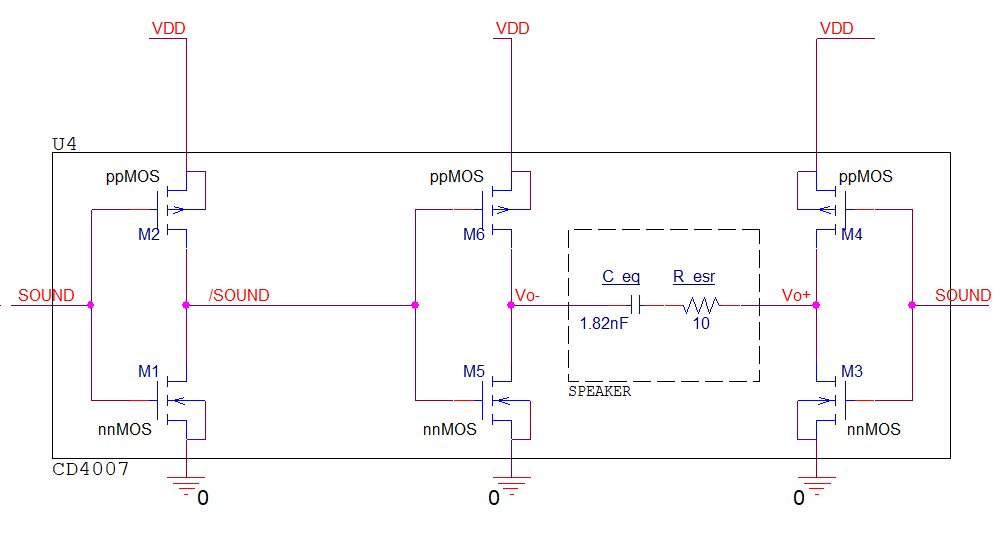
\includegraphics[width = \textwidth]{schematics/driver.png}
                \caption[]{}
            \end{figure}
            
            It is better to drive the transducer via a symmetrical wave, in order to use full swing range of the device. However, since the circuit will be powered via a 9V battery, there won’t be a negative rail. To switch the polarity of voltage an H bridge is used. 
            
            Commertially available h-bridge IC's (such as LM293) are designed for driving motors at high currents and have inferiour switching characteristics. Instead, we have decided to use CD4007, which provides three pairs of N and P MOSFETs. Two pairs are used to construct the H-bridge, and the remaining pair is used as inverter to drive the opposing column of the bridge.
        


        \subsection{Burst Generation}

            \begin{figure}[H]\centering
                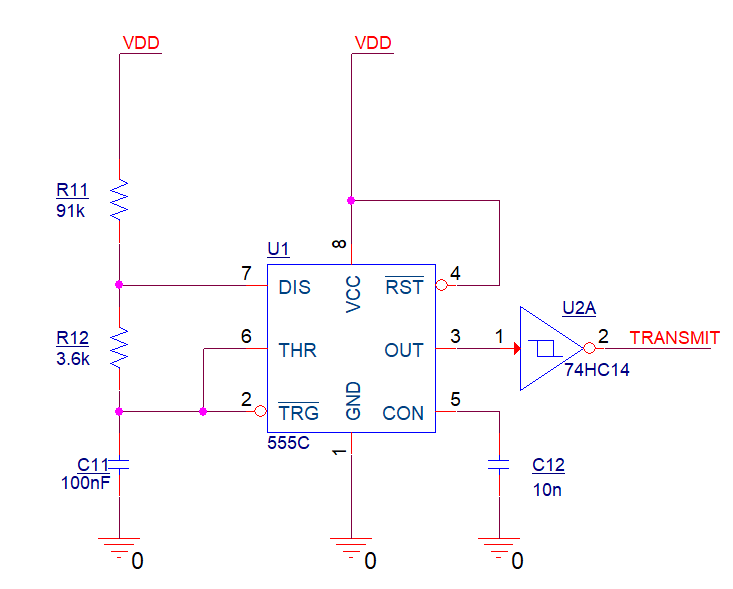
\includegraphics[width = 0.75\textwidth]{schematics/pulse_gen.png}
                \caption[]{}
            \end{figure}

            To generate the periodic pulses, another 555 timer is used, output of which will enable/disable the \SI[]{40}{\kilo\hertz} ultrasonic signal generator. During the ``on'' state of the pulse, the transmitter will be driven with ultrasonic frequencies, and during the ``off'' state, it will be kept idle. This will allow the system to accurately determine when a sound wave is sent, when the according echo is received.

            As stated previously, frequency and duty of this signal is critical, as the transmitted ultrasonic burst should contain many periods of the sound wave to be able to reliably catch the echo and convert it back into a pulse. Therefore the duty cycle should be set accordingly. 

            Similarly, the period of this pulses should be long enough to ensure that a second burst is not sent before the echo of the previous one is received to prevent mis-triggering of the counter.
            
            \bigskip
            Assuming that the longest distance to be measured is \SI{100}{\centi\metre}, and speed of sound is \SI{343}{\metre\per\second}, the echo would arrive after:

            \begin{equation}
                \texttt{max }t_f = 2 \times \frac{\SI{1}{\metre}}{\SI{343}{\metre\per\second}} = \SI{5.83}{\milli\second}
            \end{equation}

            \noindent Therefore the time between end of a pulse and start of the other should be around \SI{6}{\milli\second} minimum. For simplicity, we have decided to use \SI{150}{\hertz} pulses, corresponding to a \SI{6.67}{\milli\second} period. 

            \bigskip
            \noindent Period of the \SI{40}{\kilo\hertz} ultrasonic wave is \SI{25}{\micro\second}. Filling the pulse with 10 periods of sound wave should be sufficient for the above discussion, hence the pulse width can be set to \SI{250}{\micro\second}.

            \begin{equation}\begin{aligned}
                T = 0.693(R_A + 2R_B)C &= \num{6.67e-3} \\
                         (R_A + 2R_B)C &= \num{9.62e-3} \\
                          R_A + 2R_B   &= \num{96.2e3}
            \end{aligned}\end{equation}

            \noindent Let $C$ = \SI{100}{\nano\farad} and $R_B$ = \SI{3.6}{\kilo\ohm}

            \begin{equation}
                \implies R_A = \SI{96}{\kilo\ohm} 
            \end{equation}

            \noindent Since the period of these pulses are not of critical importance, nearest E24 value that is \SI{91}{\kilo\ohm} will be used for $R_A$.

	

        \subsection{Receiver Amplifier}

            \begin{figure}[H]\centering
                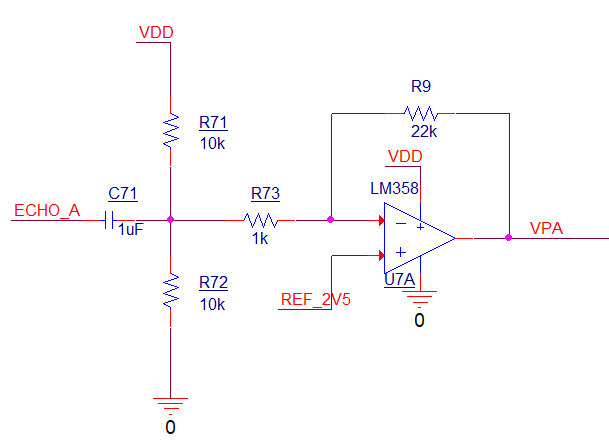
\includegraphics[width = 0.75\textwidth]{schematics/preamp.png}
                \caption[]{}
            \end{figure}

            During the transmission of the signal, it gets weaker.  On the receiver side, the received signal will most likely be small in amplitude, in order to compensate this loss, it must be amplified to be used in the following blocks. 
            
            This amplification should be made such that the lowest possible echo should not fall short of the limits of the next stage, and the highest possible amplitude echo should not exceed it.

            \bigskip
            
            To precisely recover and amplify the signal, an instrumentation amplifier would be a good choice, ho*wever, due to high prices and poor availability of instrumentation amplifiers, a commonly available general purpose opamp  (LM358) is used as amplifier instead. LM358 is selected as its the most widely available single supply opamp, even though it is far from being ideal, its GBW (gain-bandwidth product) is insufficient for this application, however, simulations showed that it works alright.

            Since the input singnal oscillates above and below zero, the negaitve rail, it is necessary to provide an offset in order not to violate input CM range of the opamp. This is done by means of a simple voltage divider, and the input signal is AC-coupled via a \SI{1}{\micro\farad} capacitor.

            Initial plan was to set the gain such that echo from the longest distance, i.e., with the lowest amplitude would still drive the opamp into saturation. However, due to the poor GBW product of the LM358, this was not possible. Instead, the gain is set as high as possible, which turned out to be around 20. 



        \subsection{Receiver Comparator}

            \begin{figure}[H]\centering
                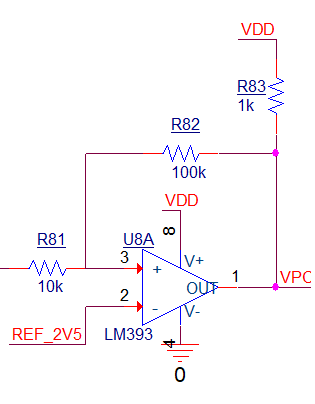
\includegraphics[width = 0.5\textwidth]{schematics/receiver_comparator.png}
                \caption[]{}
            \end{figure}

            Experiments showed that the echo can go as low as \SI{100}{\milli\volt} in amplitude for the longest distance of interest. With a gain of 20, this corresponds to about \SI{2}{\volt} amplified signal. Feeding this signal through the lowpass filter, that is the next stage, would reduce its amplitude further. To prevent this, a comparator that is able to swing to \SI{5}{\volt} is added. This addition claps the previous low amplitude signal to the rails. Another widely available general purpose device, LM393 is used for this purpose. 

            \noindent Its threshold is set to \SI{2.5}{\volt} with a hysteresis of about $V_H = \pm \SI{0.5}{\volt}$.
            
            \begin{equation}
                V_H = \pm \frac{ R_{81} } {R_{81} + R_{82} } \times V_{OUT} \approx \pm \SI{0.5}{\volt}
            \end{equation}
            
        
        \subsection{Low Pass Filter}

            \begin{figure}[H]\centering
                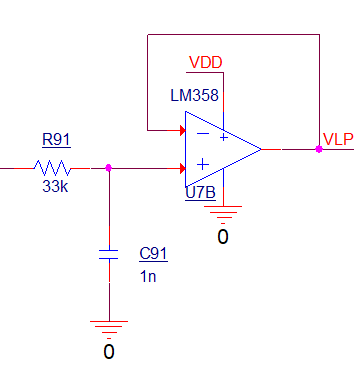
\includegraphics[width=0.5\textwidth]{schematics/lowpass.png}
                \caption[]{}
            \end{figure}
                
            Since the incoming echo signal will be a frequency modulated signal, where it consists of an ultrasonic burst filling a pulse, in order to obtain the actual waveform, it is necessary to pass the signal through a low pass filter. 
            After this stage, the ultrasonic part will be discarded and following stages will see only the outlining pulse. This LPF which is used in our design is a simple passive RC LPF.
            
            \bigskip
            A passive first order RC low pass filter is designed with corner frequency fc \~= 5kHz. Where input signal consists of a 40kHz carrier and 150 Hz \%0.3 duty pulses. Passing this signal through a LPF enables it to be further passed though a schmitt trigger and recover the digital pulse, resulting in clean fast rising and falling edges, sufficient to trigger the counter.

            \begin{equation}
                f_c = \frac{1}{2 \pi R C} = \SI{5}{\kilo\hertz} 
            \end{equation}

            \begin{equation}
                RC \approx \SI{33}{\micro\second}
            \end{equation}

            \noindent Let $C = \SI{1}{\nano\farad} \implies R = \SI{33}{\kilo\ohm}$.

        \subsection{Schmitt Trigger}

            \begin{figure}[H]\centering
                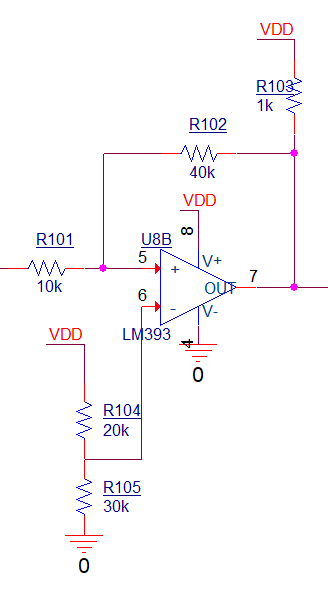
\includegraphics[width=0.5\textwidth]{schematics/schmitt.png}
                \caption[]{}
            \end{figure}
            
            After the LPF, even though the signal will resemble a pulse, it still will be an analogue signal, with slow rising/falling edges and an ambiguous amplitude value. To digitise the signal, it should be fed through a logical schmitt-trigger, output of which will be a truly digital signal. 

            Even though the amplitude value does contain information about surface type and angle, these informations are beyond the scope of this project and therefore can be discarded without any problems in this stage.

            In previous stages LM393 was used as a comparator. Since LM393 conveniently comes in dual packages, the other half is used in here. 

            As will be seen on the simulation results, output of the lowpass filter is more tricky to convert to a digital pulse. Comparator threshold is set to \SI{3}{\volt} with larges hysteresis of $\pm \SI{1}{\volt}$. This allows comparator to not trigger on leftovers of \SI{40}{\kilo\hertz} signal.

            \begin{equation}
                V_H = \pm \frac{ R_{101} } {R_{101} + R_{102} } \times V_{OUT} = \pm \SI{1}{\volt}
            \end{equation}
            

        \subsection{Counter}

            After converting the echo burst into a digital pulse, timing measurements can be done. A counter that is to be started simultaneously with the first edge of the transmitted burst, should then be stopped by the first edge of the echo signal. Output of the counter will be proportuonal to the distance. 
            
            \subsubsection{Counter Clock}

                \begin{figure}[H]\centering
                    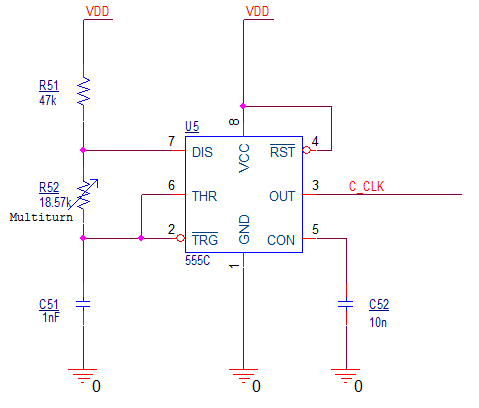
\includegraphics[width=0.75\textwidth]{schematics/counter_clock.png}
                    \caption[]{}
                \end{figure}

                By accurately setting the clock of the counter, it can be set such that for the time it takes a sound wave to travel 1 metre and back, the counter will increment by one. Hence the counter output will directly be the distance measured in centimeters. 

                Given that sound travels at \SI{343}{\metre\per\second}, an echo from \SI{1}{\centi\metre} distance would arrive after:
                
                \begin{equation}
                    t_f = 2 \times \frac{\num{1e-2}}{343} = \SI{58.3}{\micro\second}
                \end{equation}

                \noindent Therefore the clock should toggle every \SI{58.3}{\micro\second} which corresponds to a frequency of \SI{17.15}{\kilo\hertz}. 

                \bigskip
                \noindent This clock is constructed using yet another 555 IC. Using the equations provided on the datasheet for astable mode of operation:
                
                \begin{equation}\begin{aligned}
                    T = 0.693(R_A + 2R_B)C &= \num{58.3e-6} \\
                            (R_A + 2R_B)C &= \num{84.13e-6} \\
                            R_A + 2R_B   &= \num{84.13e3}
                \end{aligned}\end{equation}

                \noindent Let $C$ = \SI{1}{\nano\farad} and $R_A$ = \SI{47}{\kilo\ohm}

                \begin{equation}
                    \implies R_B = \SI{18.57}{\kilo\ohm} 
                \end{equation}

                \noindent As stated before, accuracy of this clock is important, and a multiturn trimpot can be used in series with the $R_B$ to precisely set the frequency.

            \subsubsection{Counter/7-Segment Driver}

                \begin{figure}[H]\centering
                    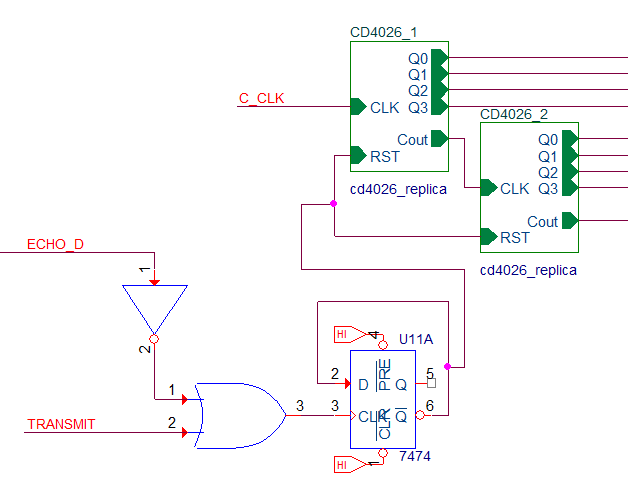
\includegraphics[width=\textwidth]{schematics/counter.png}
                    \caption[]{}
                \end{figure}

                As for the counter itself, CD4026 is perfect for the job. It is a BCD counter with 7-Segment driving outputs, and a carry out pin. By using the built in carry out pin, two CD4026's can be cascaded such that the carry of the less significant BCD digit will drive the clock of the more significant BCD digit. 

                Note that given schematic is not an actual model for CD4026. To be able to make sense of the counter output during simulations, we have replicated CD4026 in such a way that it outputs in BCD instead of 7-Segment decoded outputs. In reality, CD4026 would have 8 outputs driving corresponding segments on the display.

            \subsubsection{Triggering the Counter}

                \begin{figure}[H]\centering
                    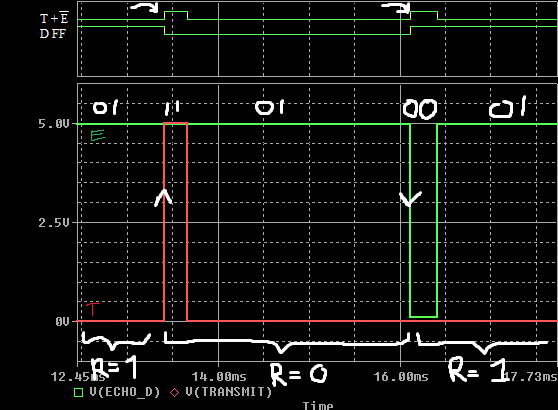
\includegraphics[width=\textwidth]{reset_problem.png}
                    \caption[]{}
                \end{figure}
                    
                As previously described, counter should be started at first edges of ``TRANSMIT'' pulses, (see section 4.3, ``Burst Generation'') and stopped at the first edges of the received echos. Such that it will be counting during the ``listening'' period, where the device is waiting for echo to arrive. 
                
                Note that the amplified and processed echo signal is active low, and transmit signal is active high. Therefore, counter should be started at the rising edge of the ``TRANSMIT'' and stopped at falling edge of ``ECHO''. Unfortunately, this is not possible using simple combinational logic elements, since different outputs are required for the same input states, as can be seen from the figure. 

                Instead, the circuit requires an edge sensitivity. As can be seen from the figure, OR'ing these two signals results in two rising edges in the necessary points in time, however, CD4026 is level sensitive. Therefore it is necessary to convert this edge based information back to a level based information. This is done by means of a D flip flop in astable multivibrator mode.



	    

    \pagebreak
    \section{Results}
        
        \noindent Following simulations are conducted in OrCAD PSpice. 

        \subsection{Transmitter Side Partial Simulations}

            \subsubsection{Sound Burst Generation}

                \noindent Showing ``TRANSMIT'' pulses (red) and the \SI{40}{\kilo\hertz} ultrasonic sound wave filling in them (green) at two different time scales. It can be seen that the pulse is successfully filled with ultrasonic frequency signal. One small deformation is that the first pulse is slightly longer and the last is slightly shorter in time. This is due to the inevitable internal delayed response to the reset pin of 555, and it should not constitute a problem.

                \begin{figure}[H]\centering
                    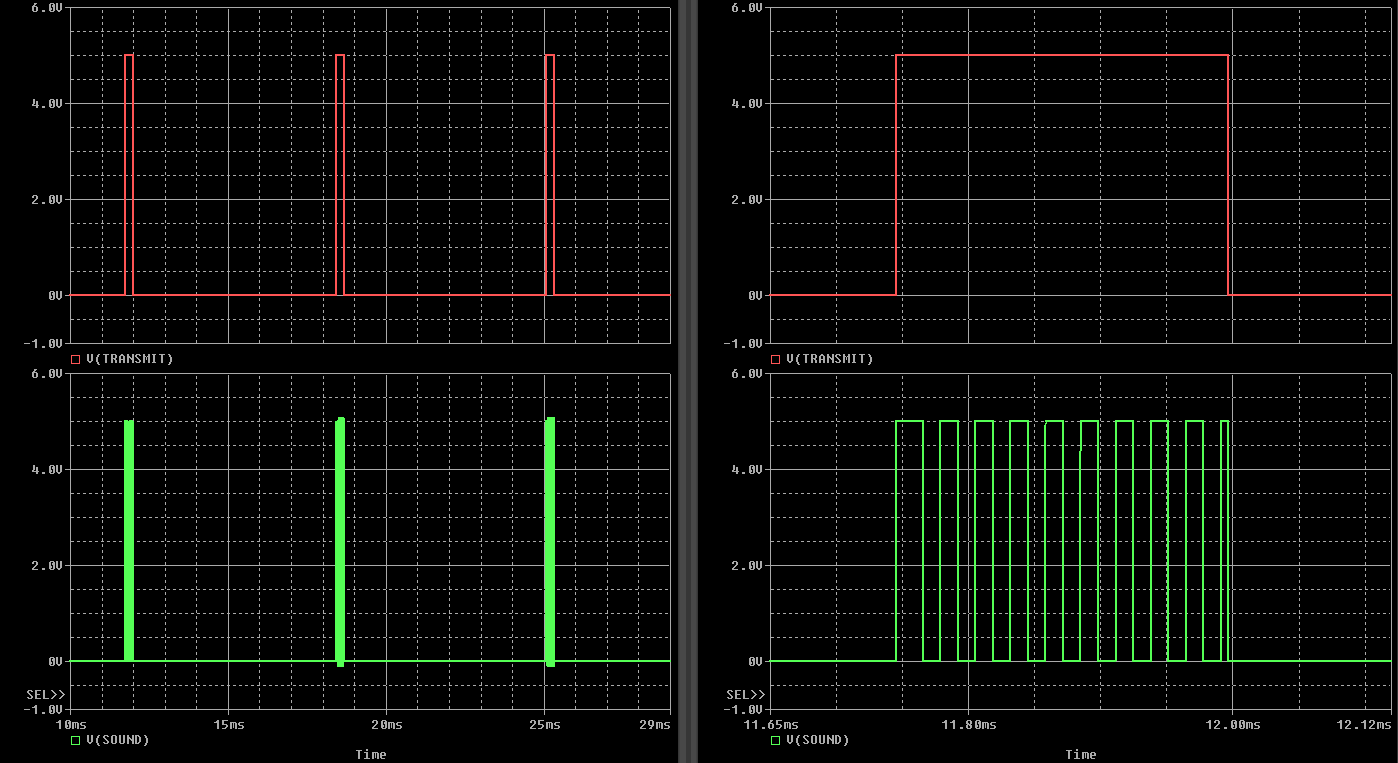
\includegraphics[width = \textwidth]{simulations/transmit/burst_and_ultra.png}
                    \caption[]{}
                \end{figure}
            
            \pagebreak
            \subsubsection{Driver}

                \noindent Converting previous logic level burst signal (red) into $\pm \SI{5}{\volt}$ symmetric wave for driving the transmitter (green). 
                \begin{figure}[H]\centering
                    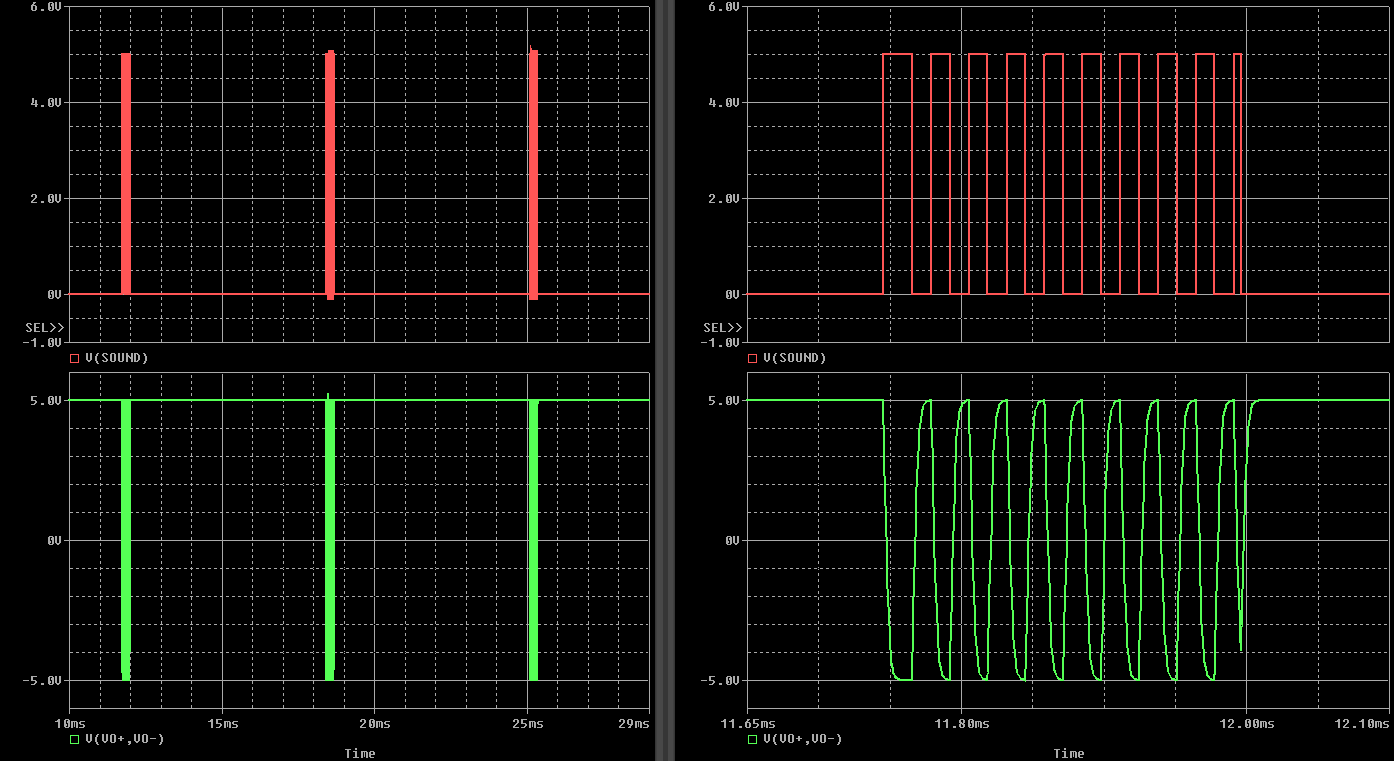
\includegraphics[width = \textwidth]{simulations/transmit/driver.png}
                    \caption[]{}
                \end{figure}

                A model of the speaker was attached to the output of the driver during this simulation. Experiments had shown that the transmitter used was a capacitive spekaer with capacitance of \SI{1.82}{\nano\farad}. This inevitably deforms the signal slightly and the capacitor charge/discharge curves can be seen on the output.

            \pagebreak
            \subsection{Travelling Echo Simulation}

                \begin{figure}[H]\centering
                    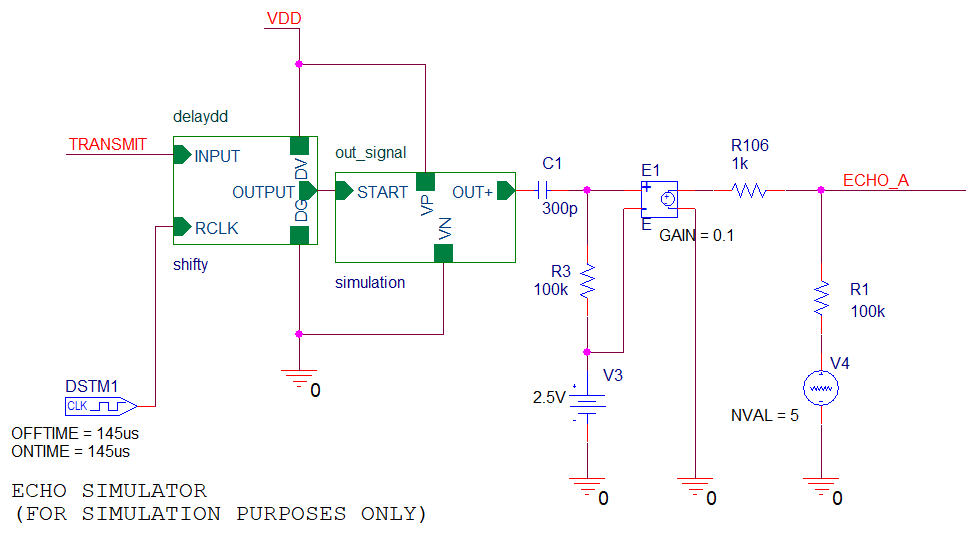
\includegraphics[width = \textwidth]{schematics/echo_sim.png}
                    \caption[]{}
                \end{figure}

                Received echo signal will be the delayed, attenuated and noisy version of the transmitted signal. In order to simulate these effects, following circuit is constructed. This is only to be able to simulate the entire system at once, and is not a part of the actual design.

                To achieve delay, \SI{40}{\kilo\hertz} generator is duplicated. Output of the ``Burst Generator'' circuit, ,i.e.,``TRANSMIT'' signal that is responsible for starting the transmission by enabling the actual ultrasonic generator, is also passed through a 10 bit shift register made using D flip flops and fed to this duplicated ultrasonic generator. By setting the clock of the register accordingly, duplicated ultrasonic generator can be set to trigger with a controlled amount of delay. 

                To achieve attenuation, a voltage controlled voltage source is added with adjustable gain, smaller than 1.

                To simulate noise, a random noise source is added with noise magnitude of 5V. This noise source is coupled into the signal source that has \SI{1}{\kilo\ohm} series resistance using \SI{100}{\kilo\ohm} resistor, providing an SNR of 100.

                \pagebreak
                Below, the construction of the shift register and its outout is shown. It can be seen that the device delays the input for roughly 10 clock cycles.      

                \begin{figure}[H]\centering
                    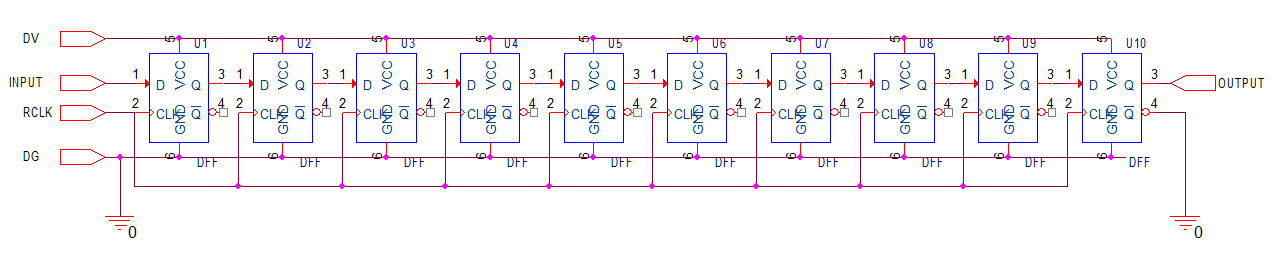
\includegraphics[width = \textwidth]{schematics/shifty.png}
                    \caption[]{}
                \end{figure}

                \begin{figure}[H]\centering
                    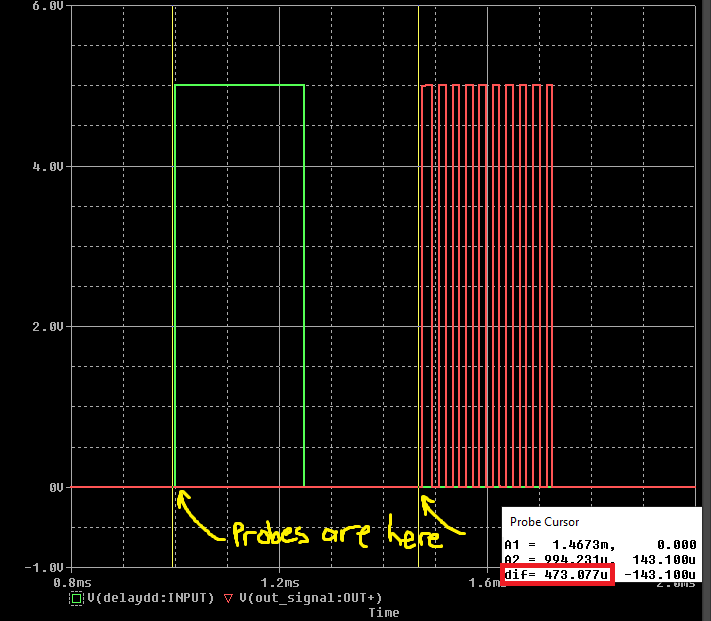
\includegraphics[width = 0.75\textwidth]{simulations/echo_large.png}
                    \caption[]{}
                \end{figure}



        \pagebreak
        \subsection{Receiver Side Partial Simulations}
                
                To better control the simulation environment, following simulations are done seperately from the transmitter side and echo simulations. Input is generated using an ideal pulse source, coupled with a noise source, instead of the method described on the previous section, which was created to simulate entire system.

                Receiver side circuitry itself is simulated as a whole, for all the simulations in this section, output of one stage is input of the next one.

                \bigskip\bigskip

            \subsubsection{Preamplifier}

                \noindent Low amplitude, noisy echo signal (upper) and output of the preamplifier (lower). It can be seen that the amplified signal still is relatively low in amplitude, with approximately \SI{1}{\volt} amplitude for \SI{100}{\milli\volt} input signal, even though the gain is set to 20. This is the result of the poor GBW product of the LM358.
                \begin{figure}[H]\centering
                    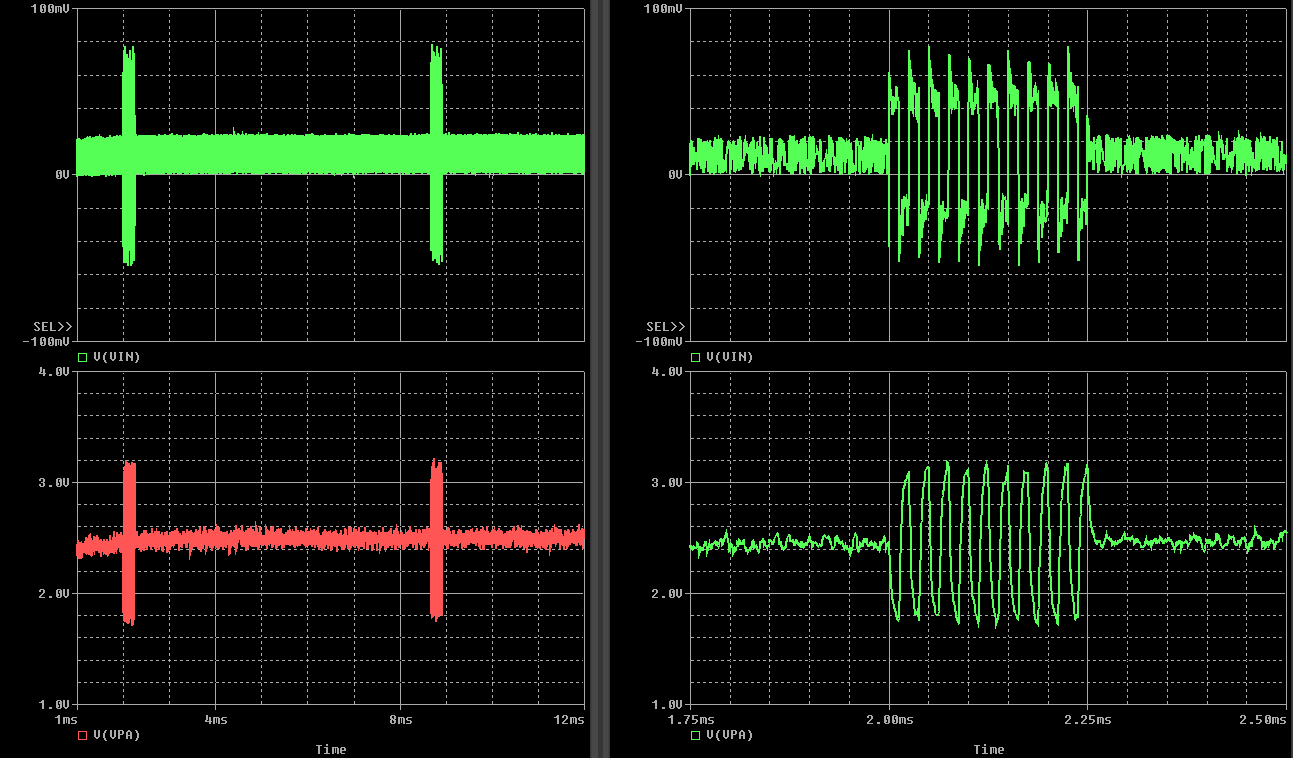
\includegraphics[width = \textwidth]{simulations/receive/preamp.png}
                    \caption[]{}
                \end{figure}

            \pagebreak
            \subsubsection{Receiver Comparator}
                \noindent Clamping the relatively low amplitude preamplified signal to the supply rails. It can be seen that the signal is effectively amplified using the comparator. Also there are no multiple-crossings even in this lowest possible amplitude of interest for the input signal. 

                \begin{figure}[H]\centering
                    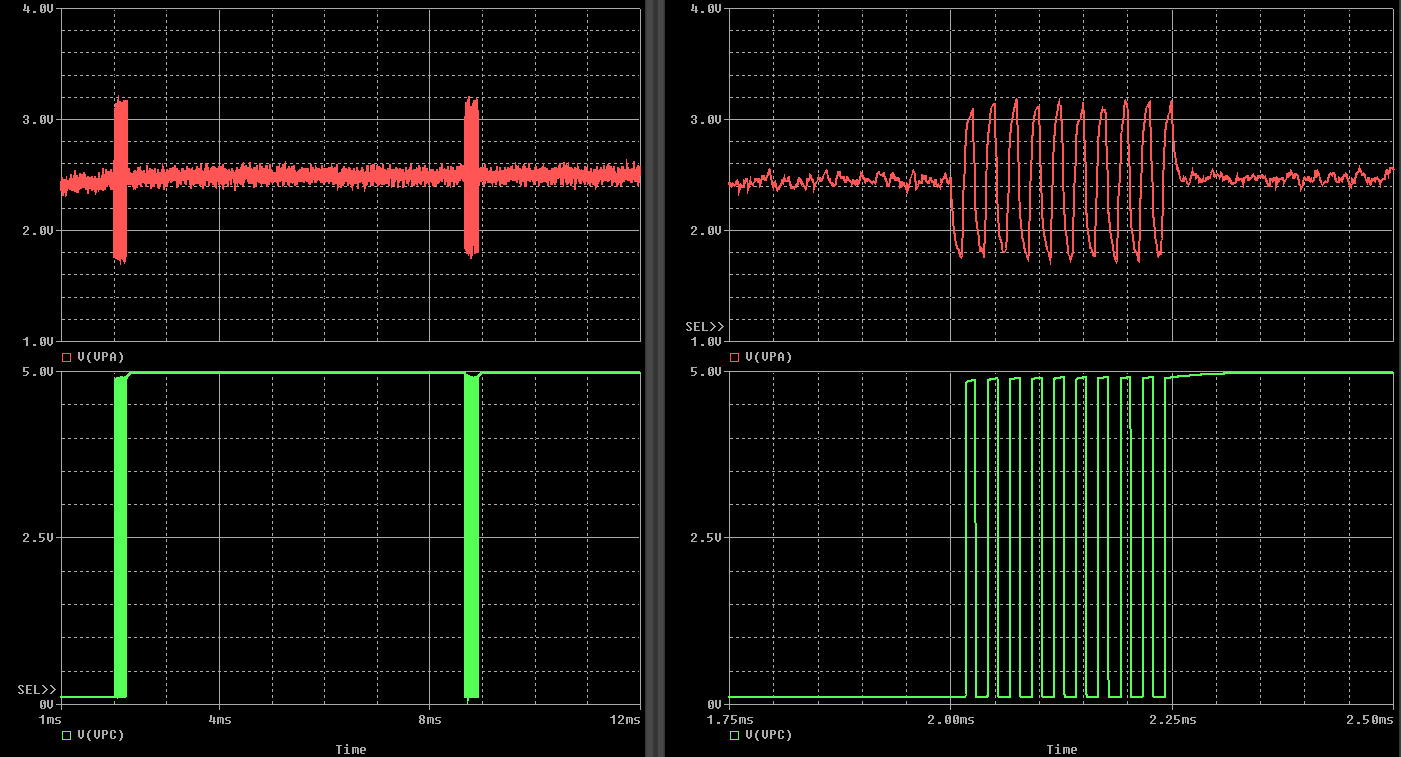
\includegraphics[width = \textwidth]{simulations/receive/preamp_comparator.png}
                    \caption[]{}
                \end{figure}
            
            \pagebreak
            \subsubsection{Lowpass Filter}
                \noindent Filtering the \SI{40}{\kilo\hertz} signal out. It can be seen that the simple passive RC lowpass filter isn't doing a great job, signal dopped in half in amplitude and still contains a singificant amount of \SI{40}{\kilo\hertz} ``noise'', but it suffices for the next stage to be able to handle it.

                \begin{figure}[H]\centering
                    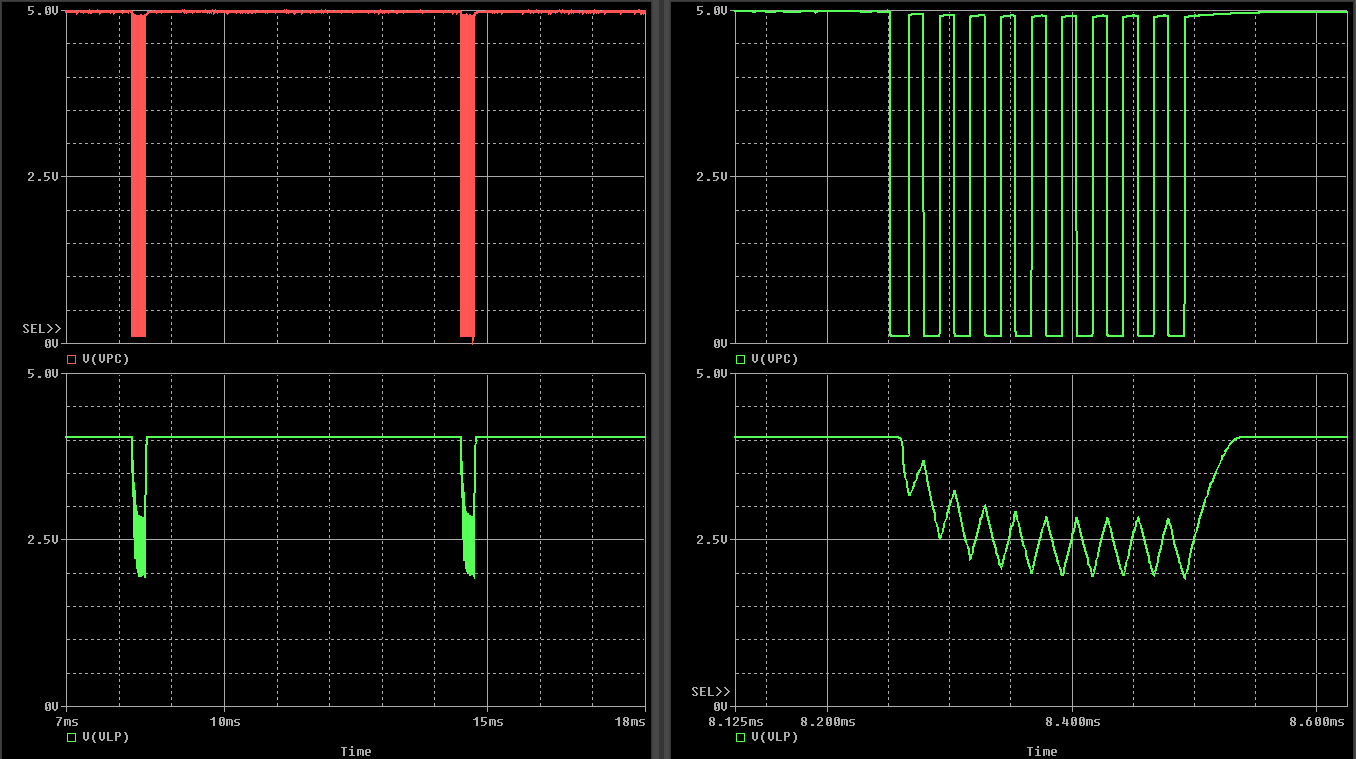
\includegraphics[width = \textwidth]{simulations/receive/lpf.png}
                    \caption[]{}
                \end{figure}
            
            \pagebreak
            \subsubsection{Schmitt Trigger}
                \noindent Finally, using a schmitt trigger with relatively large hysteresis, (\SI{3}{\volt} threshold with $\pm \SI{1}{\volt}$ hysteresis) filtered signal is converted into a logic level pulse.

                \begin{figure}[H]\centering
                    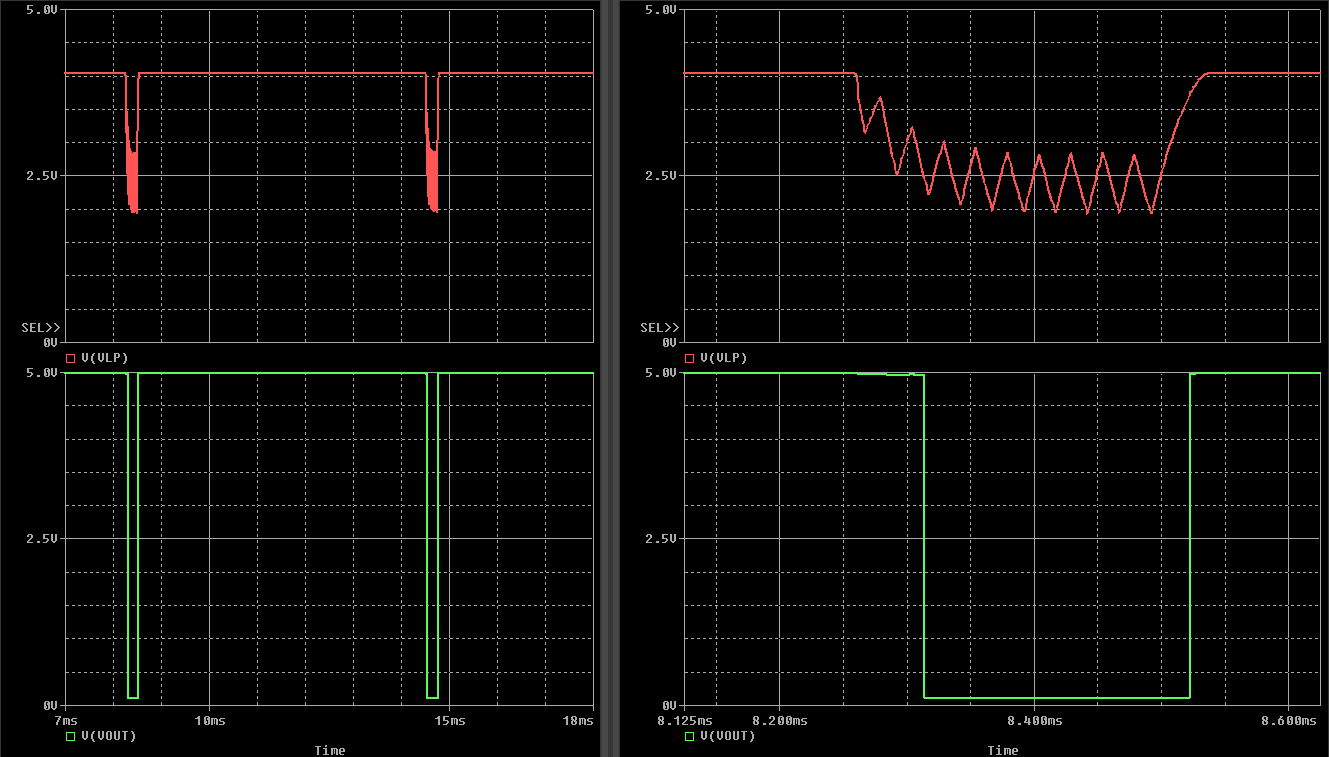
\includegraphics[width = \textwidth]{simulations/receive/schmitt.png}
                    \caption[]{}
                \end{figure}
       
        
        \pagebreak
        \subsection{Complete System Simulation}

            Entire design is simulated as a whole, using the echo simulating subcircuitry to simulate the sound wave travelling on air, reflecting back and getting picked up by the microphone. Clock of the delay line is set to create a delay  approximately \SI{50}{\centi\metre}, although measuring the actual delay showed that the echo was delayed corresponding to \SI{46}{\centi\meter}, (measured delay between transmitted and received pulses read \SI{2.7}{\milli\second} at the right window.). Therefore we expect the counter to read 46.  

            \noindent Amplitude of the incoming echo is set to about \SI{600}{\milli\volt}, which is how large we expect echo signal to be from \SI{50}{\centi\meter} based on our previous experiments.


            At the top left corner, ultrasonic sound burst driving the speaker is shown in green. At bottom left in red, picked up echo is shown. At bottom right corner, sent pulse (green) and reconstructed echo pulse (red) are shown, as well as the time delay between them. Finally at the upper left corner, counter outputs can be seen. Bits that are enclosed by white rectangles are arranged to be read from bottom up. Keep in mind that the representation is in BCD, not binary. 

            Output reads \texttt{0100 0110} in BCD, which suggests that the measured distance is \SI{46}{\centi\metre} which is exactly correct. Second from the bottom bit shows that carry-out bit has not been set, indicating that the distance is in-range. 

            \bigskip
            
            \begin{figure}[H]\centering
                \makebox[\linewidth]
                    {
                        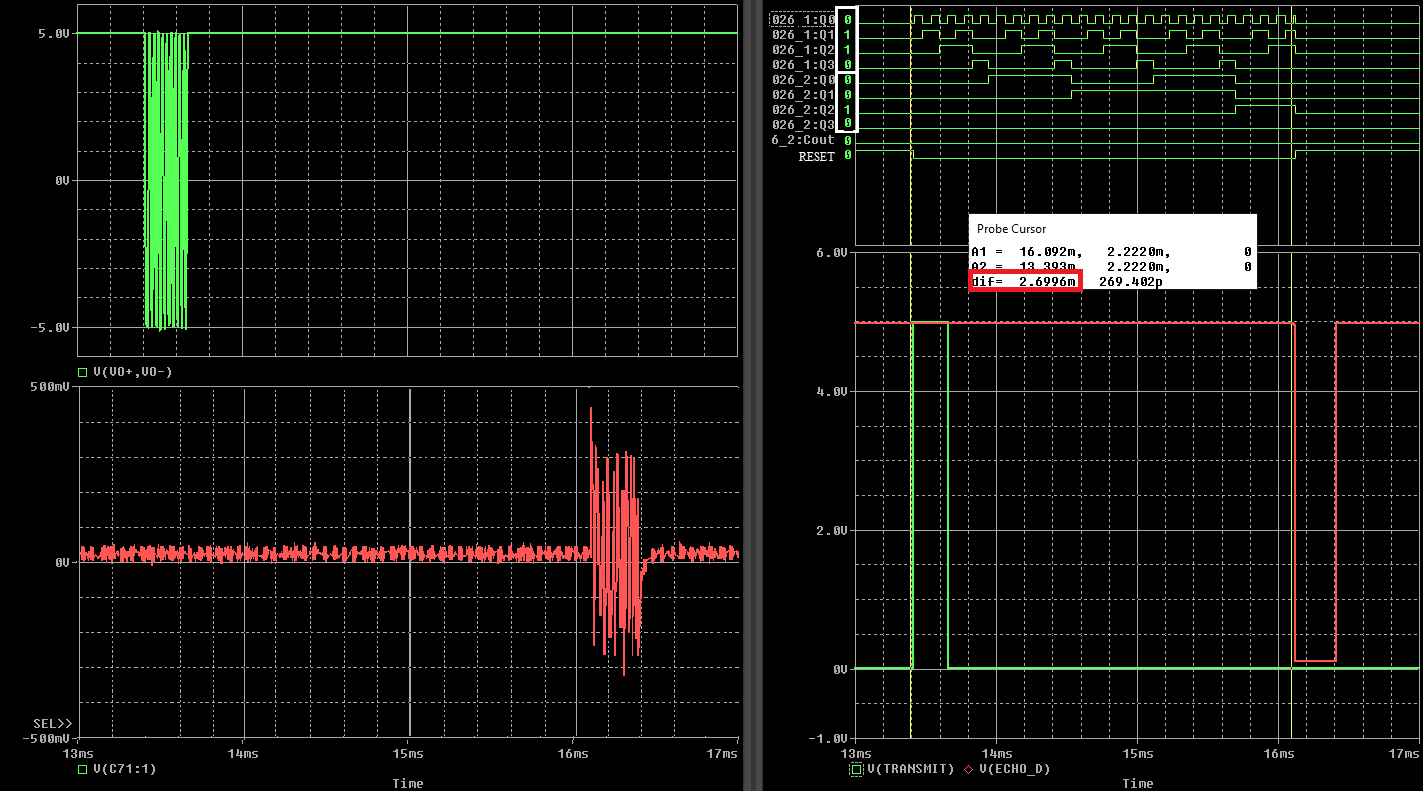
\includegraphics[width=1.25\linewidth]{simulations/complete.png}
                    }
                    \caption[]{}
            \end{figure}

            
    \pagebreak
    \section{BOM List}
        \begin{figure}[H]\centering
            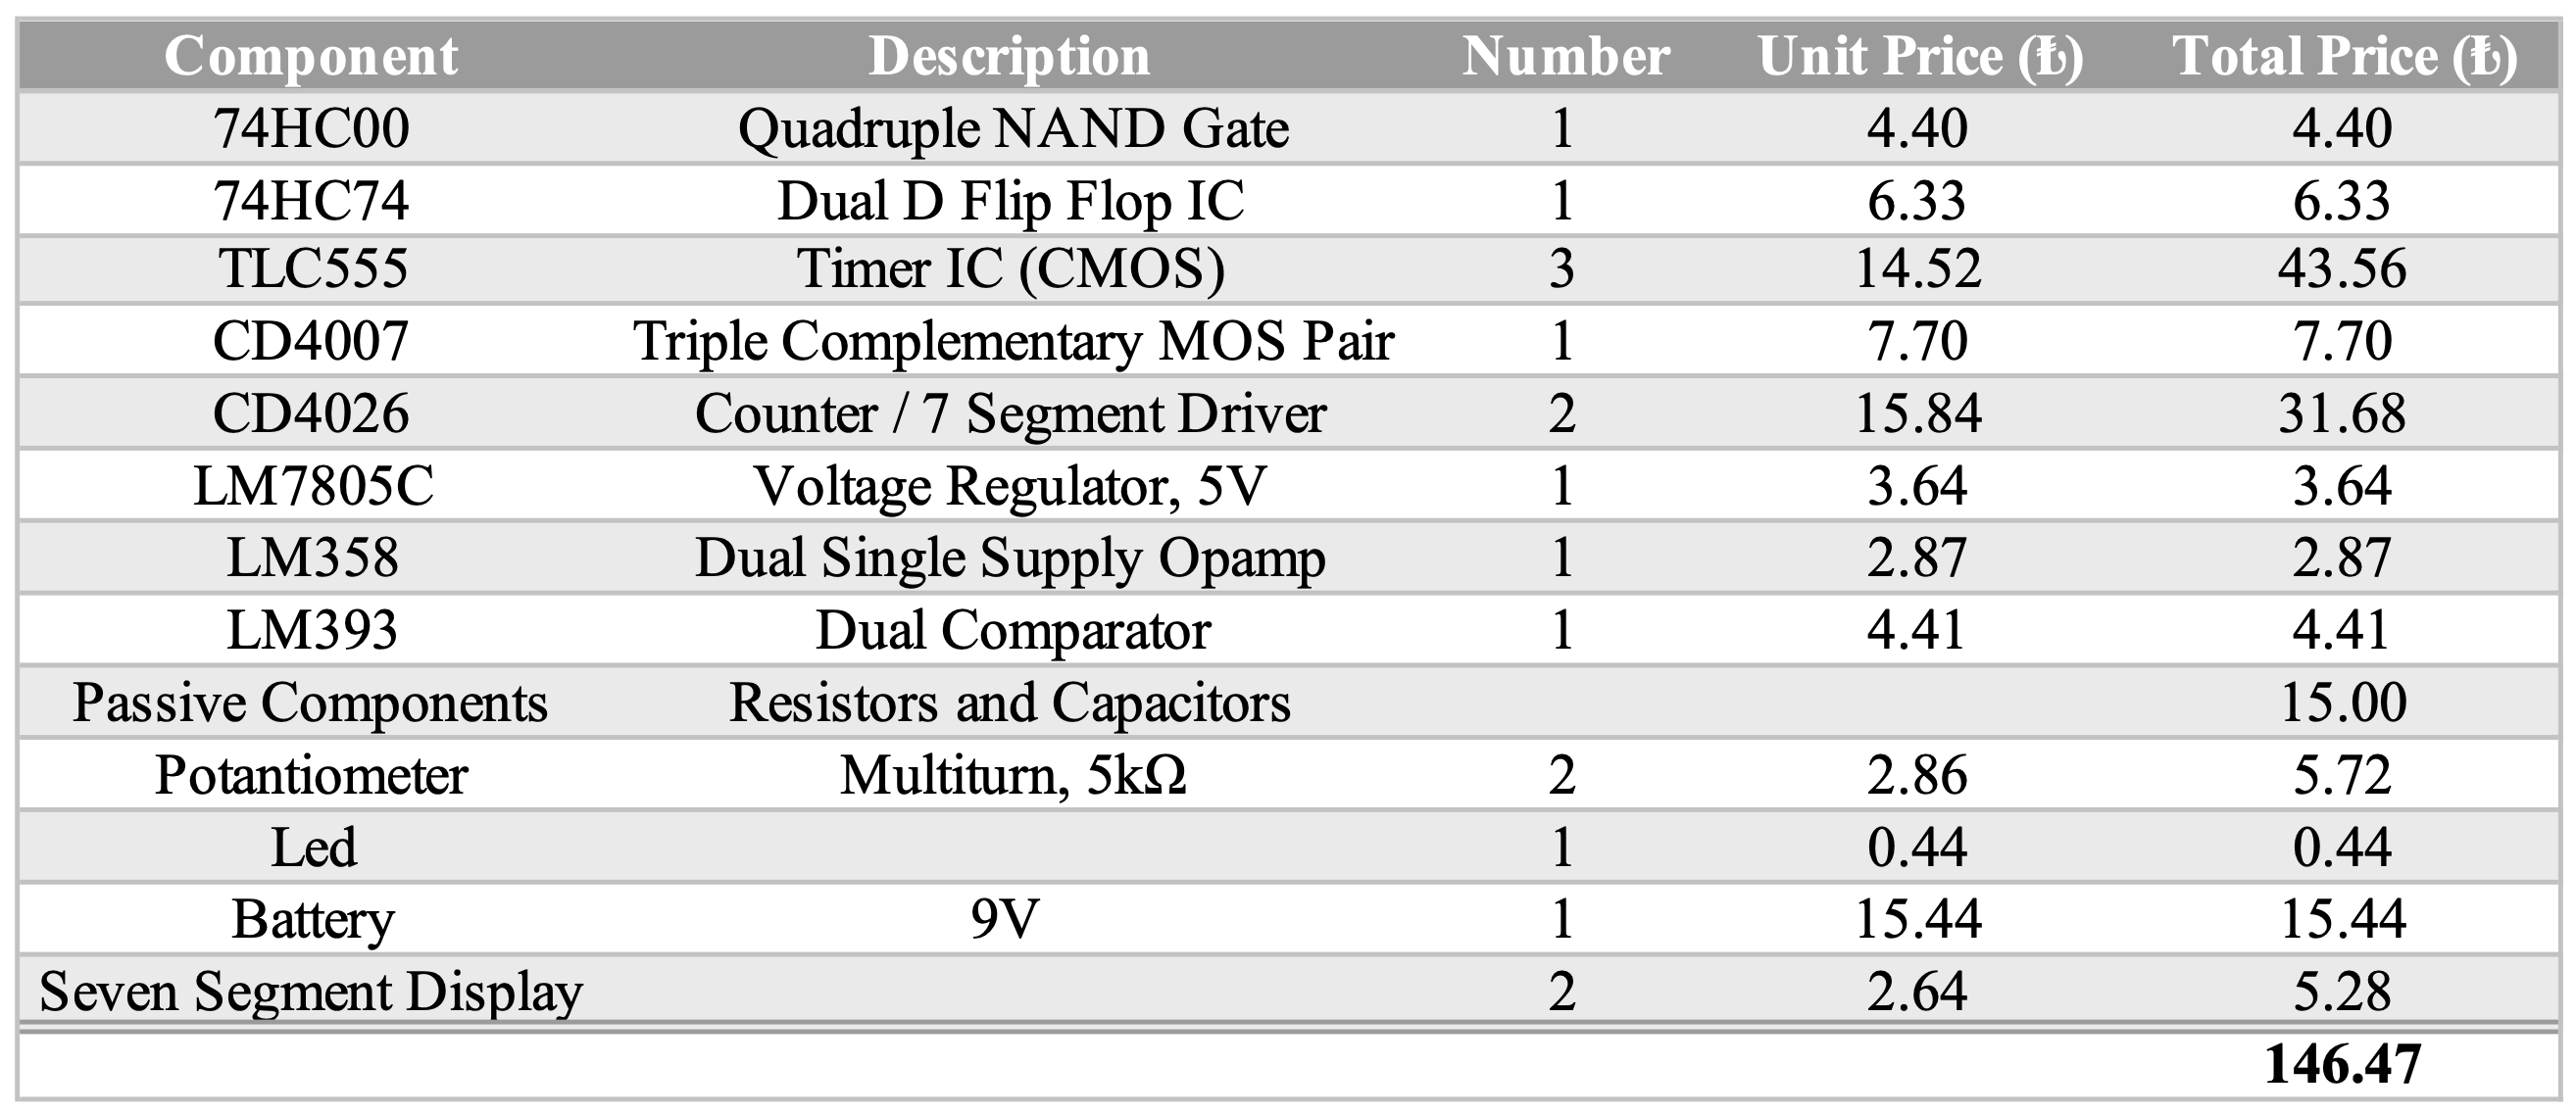
\includegraphics[width = \textwidth]{bom.png}
        \end{figure}

      
    \pagebreak
    \section{Conclusion}
    
        As mentioned in the Ultrasonic Frequency Synthesis section (section 4), HCSR04 drives the transducers with a symmetrical wave. The first design idea that came to our mind to accomplish this is to use  two square waves with 180 degree phase difference to drive each pin of the transducer. Such that, one pin of the transducer will be kept on 0V where the other is kept at 5V. By alternating this process between the two pins, a differential symmetric 10V square wave can be obtained as shown in figure.
        
        To implement this idea to the circuit, two 555 ICs will be driven on monostable mode with 0.25 duty cycle. To synchronise two pulse generators, each IC will be triggered by the falling edge of the other. As a result, a fully differential square wave with twice the frequency of individual pulse generators will be obtained.
        
        The reason why this circuit, which we have already designed, is not realized is the trigger pulse must be shorter than the desired
        $t_H$. In our design, since the output of the first 555 comes to the trigger pin of the other 555, it does not comply with this condition.
    
        \bigskip
        For the receiver side, LM358 comes with a lot of shortcomings, it is single-suppy, but not rail-to-rail, which causes output to saturate at \SI{4}{\volt} instead of 5. Combined with very poor GBW product, preamplifier fails to amplify the input signal to sufficient levels. We have added more blocks such as the comparator following the preamplifier, inevitably complicating the circuit. Even though the simulation seems to work pretty decently, we still have our doubts when in comes to building the circuit. 

        \bigskip
        We have imperically estimated how noisy and low in amplitude the echo signal will be and tried to model it in the simulations as close to results as possible, by running the simulation with even lower amplitudes, and with heavy noise. By running simulations under these worst conditions, we have fine-tuned the design, until the point where the worst case simulation succeeded.

        \bigskip
        Simulating the echo was perhaps one of the hardest parts of the simulation process. An accurate echo simulation is very important, since this is the primary input of the system. After many failed attempts to syncronise transmitting and receiving side of the circuit, we have finally managed to accurately simulate the receiver picking up the delayed echo from the transmitter. This allowed us to simulate the entire system as a whole, and confirm its function.
        
        \bigskip
        One major and fatal problem of the design is that the display inputs are not buffered. Given that the counter starts from zero and counts up to the measured distance in at most few milli seconds and then goes back to zero means that the user will have few milliseconds to read the display. We have not realized this problem until the final simulations. Problem can be solved simply by adding a register and refreshing it after the counter is done. Register will hold its values until the next refresh cycle has come, and the display will be off for at most few milli seconds. This addition will be documented at the final report. 

     
    \pagebreak
    \section{Gannt Chart}

        \begin{figure}[H]\centering
            \makebox[\linewidth]
                {
                    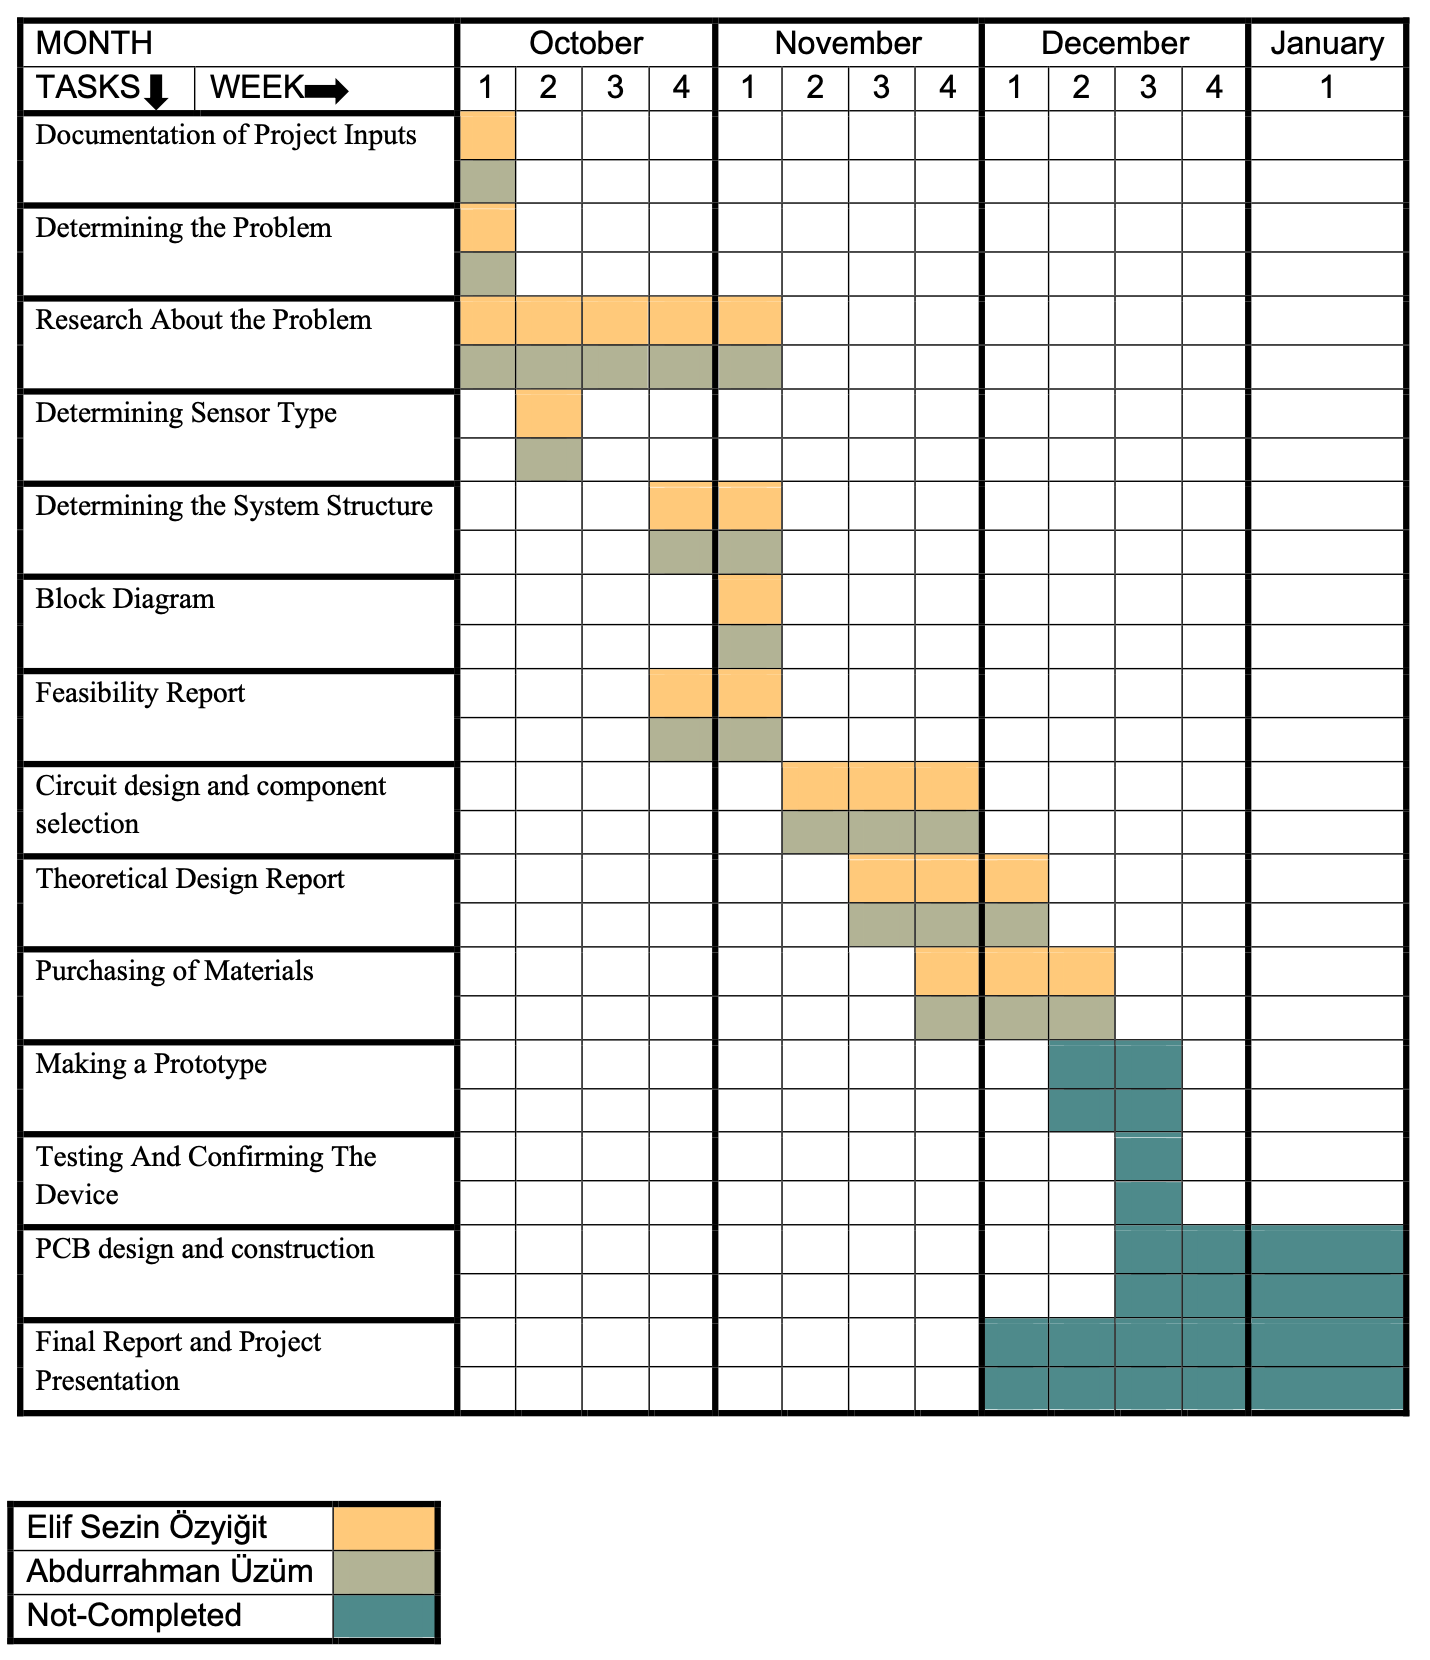
\includegraphics[width=1.2\linewidth]{Gantt_Chart_v2.png}
                }
                \caption{Gannt Chart}
        \end{figure}



    


    \begin{thebibliography}{}	
        
        \bibitem{}
        \textit{Mubina Toa, Akeem Whitehead}, \textbf{\textit{``Ultrasonic Sensing Basics''}}, Texas Instruments

        \bibitem{}
        \textit{Akeem Whitehead}, \textbf{\textit{``GA460 Ultrasonic Module Hardware and SoftwareOptimization''}}, Texas Instruments

        \bibitem{}
        \textit{Paul Horowitz, Winfield Hill}, \textbf{\textit{``The Art of Electronics''}}, Cambridge University Press

        \bibitem{}
        \textbf{\textit{``Single Supply Op Amp Design Techniques''}}, Texas Instruments
        
        \bibitem{}
        \textbf{\textit{``Single Supply Operational Amplifiers''}}, Burr-Brown


    \end{thebibliography}
            





\end{document}